\chapter{线性空间}
\begin{center}
	% \textcolor[RGB]{255, 0, 0}{\faHeart}越想贴近事实,不明白的事情就越多.\textcolor[RGB]{255, 0, 0}{\faHeart}
	「越想贴近事实,不明白的事情就越多」
\end{center}
\rightline{——《宝石之国》}
\vspace{-5pt}
\begin{center}
	\pgfornament[width=0.36\linewidth,color=lsp]{88}
\end{center}

\section{标量与向量}

\subsection{数的运算}

从小学一年级开始我们就接触了整数,并且学会进行加减乘除;长大一些后,我们了解到了分数,将数系扩充到了有理数部分;再后来初中阶段我们遇到了平方根这种运算,接触到了无理数,我们把这些数都统称为实数,后来我们又了解了 $-1$ 也能被开平方根,开创了复数领域;同时在高中阶段,我们也学习了简单的集合论,通常我们会用几个记号来表示这些数域。

\begin{definition}{数集的符号}
	这些数集有着相对应的符号:
	\begin{itemize}
		\item $\mathbb{N}$ 表示所有自然数的集合,其元素是所有非负整数。
		\item $\mathbb{Z}$ 表示所有整数的集合。
		\item $\mathbb{Q}$ 表示所有有理数的集合,其中有理数被定义为所有能够表示为 $\frac{m}{n},m\in \mathbb{Z},n\in \mathbb{Z}$ 的数。
		\item $\mathbb{R}$ 表示所有实数的集合。
		\item $\mathbb{C}$ 表示所有复数的集合。
	\end{itemize}
\end{definition}
%此外,德国数学家Frobenius也证明,在当下的数学体系中 $\mathbb{C}$ 是最大的数域,

由于这门课不是实分析或高等代数,所以不会详细讲解这些数集怎么构造,读者只需要对此有一个简单的认识就可以了。众所周知,数的运算分别有加减乘除四种,如果读者觉得自己小学数学不错的话,一定知道下面的定理。

\begin{axiom}{域公理}
	对于这些数的基本算数性质有:
	\begin{enumerate}
		\item \textbf{交换律(communitativity)}:对于所有的$\alpha,\beta \in \mathbb{C}$有$\alpha+\beta=\beta+\alpha,\alpha\beta=\beta\alpha$;
		\item \textbf{结合律(associativity)}:对于所有的$\alpha,\beta,\gamma \in \mathbb{C}$有$(\alpha+\beta)+\gamma=\alpha+(\beta+\gamma),(\alpha\beta)\gamma=\alpha(\beta\gamma)$;
		\item \textbf{单位元(identities)}:对于所有的$\lambda \in \mathbb{C}$都有$\lambda+0=\lambda,1\lambda=\lambda$;
		\item \textbf{加法逆元(additive inverse)}:对于所有的$\alpha \in \mathbb{C}$都存在唯一的$\beta \in \mathbb{C}$使得$\alpha+\beta=0$;
		\item \textbf{乘法逆元(multiplicative inverse)}:对于每个$\alpha \in\mathbb{C}$且$\alpha\neq 0$,都存在唯一的$\beta \in \mathbb{C}$使得$\alpha\beta=1$;
		\item \textbf{分配律(distributive)}:对于所有的$\alpha,\beta,\gamma \in \mathbb{C}$都有对于所有的$\alpha(\beta+\gamma)=\alpha\beta +\alpha\gamma$.
	\end{enumerate}
\end{axiom}

如果一个数域$\mathbb{F}$和$\mathbb{C}$一样满足上述性质,我们称$\mathbb{F}$中的元素为标量(scalar),当然$\mathbb{C}$和$\mathbb{R}$的所有元素也是标量。

\subsection{标量}

如上所述,标量通常强调的是,这一个元素是一个数,而不是向量(稍后给出定义),实际上只是``数''的一种花里胡哨的叫法而已。德国数学家Frobenius 已经证明,当下数学体系内再也没有比$\mathbb{C}$更大的数系了,所以我们可以称对于每一个$\alpha \in \mathbb{C}$,$\alpha$是标量,例如 $3+4\mathrm{i}$ 是一个标量。

\begin{example}
	前文所述,我们说过复数是最大的数系,请求出$\sqrt{\mathrm{i}}$的两个解,其中$\mathrm{i}=\sqrt{-1}$。
	\tcblower
	\textcolor{purple}{\textbf{解}}:设$\sqrt{\mathrm{i}}=z=(a+b\mathrm{i})$,其中$a,b \in \mathbb{R}$,通过两边将其平方可得$$\mathrm{i}=(a+b\mathrm{i})^2=a^2-b^2+2ab\mathrm{i}$$观察式子联立方程组为$$\left\{\begin{matrix} 
		a^2-b^2=0 \\  
		2ab=1
	\end{matrix}\right. $$
	解此方程组可得$$\left\{\begin{matrix} 
		a=b \\ 
		a=\pm \frac{\sqrt{2} }{2} 
	\end{matrix}\right. $$
	所以$\sqrt{\mathrm{i}}$的两个解为$$z_1=\frac{\sqrt{2}}{2}+\frac{\sqrt{2}}{2}\mathrm{i},z_2=-\frac{\sqrt{2}}{2}-\frac{\sqrt{2}}{2}\mathrm{i}$$
\end{example}

\subsection{元组}

若$n\in \mathbb{N}$,我们将由$n$个数按顺序排列成为的一个组称之为元组(tuple),通常的记法为:有小括号包含这$n$个数,且有序排列,中间由逗号隔开,例如$(a,b)$是一个长度为2的元组,如果长度为$n$且由$z_1,z_2,z_3,\cdots,z_n$这些数组成的元组的记法可能如下所示:$\left( z_1,z_2,z_3,\cdots,z_n\right) $。

\begin{ascolorbox1}{思考}
	集合是元组吗?
\end{ascolorbox1}

对于这个思考题,很显然答案是不对的,因为元组强调以下两点:
\begin{itemize}
	\item 有序性,$(3,5)$和$(5,3)$并不相等,而$\{3,5\}$和$\{5,3\}$是相等的集合;
	\item 可重复,$(3,3)$和$(3,3,3)$并不相等,而$\{3,3\}$和$\{3,3,3\}$是相等的集合,它们等同于$\{3\}$。
\end{itemize}

\subsection{笛卡尔积}

接下来我们慢慢引入向量的概念,在讲向量之前,笔者想和大家谈一谈如何生成这样的空间来容纳我们向量的概念,这里有一个定义叫做笛卡尔积(Cartesian product)。

\begin{definition}{笛卡尔积}
	\label{def:dicar}
	两个集合${\displaystyle X}$和${\displaystyle Y}$的笛卡尔积是所有可能的有序对组成的集合,其中有序对的第一个对象是$X$的成员,第二个对象是$Y$的成员,记作:$${\displaystyle X\times Y := \footnote{符号$:=$表示定义为,用来明确地给某个符号或概念赋予一个新的定义,例如:妈妈$:=$养育与教养子女成长的女性} \left\{\left(x,y\right)\mid x\in X \text{且} y\in Y\right\}}$$
\end{definition}

举个很常见的例子,如果集合$X$是13个元素的点数集合${\displaystyle \left\{A,K,Q,J,10,9,8,7,6,5,4,3,2\right\}}$而集合$Y$是四种花色$\{\spadesuit, \heartsuit, \diamondsuit, \clubsuit\}$,则这两个集合的笛卡尔积是有52个元素的标准扑克牌的集合:$$X\times Y = \left\lbrace (A,\spadesuit),(K,\spadesuit),(Q,\spadesuit)\cdots (2,\spadesuit),\cdots,(3,\clubsuit),(2,\clubsuit)\right\rbrace $$

\subsection{空间 $\mathbb{F}^n$}

我们定义$\mathbb{R}^2=\mathbb{R} \times \mathbb{R}$,根据笛卡尔积的运算规则,集合$\mathbb{R}^2$为所有有序实数2元组构成,即$$\mathbb{R}^2=\{(x,y)\mid x,y \in \mathbb{R}\}$$在现实生活中,我们可以将它看成是一个二维平面,而$\mathbb{R}^3$在现实生活中,我们可以将它看成是一个三维空间。

我们上述提到集合$\mathbb{F}$内的元素是一个标量,那么$\mathbb{F}^n$则由无数个的$n$元组构成,例如$\mathbb{C}^6$就是含有6个有序元素构成的一个空间,虽然当$n>3$的时候在实际生活中想象它们绝非易事,但是数学就是一门由具体到抽象的科目,我们可以使用类比的手法,让它们和在$\mathbb{R}^2$与$\mathbb{R}^3$上运算一样有自己的实际意义。

\subsection{向量}

如之前所述,我们终于提到了向量(vector)这个概念,只不过可能会令读者失望的是,数学科目上的向量是一个非常抽象的东西,那么我们把目光转换到另外一门和数学紧密相关的科目上:物理。

学基础物理的学生总是很实际,他们将数学转化为解决现实生活中问题的工具,所以在他们眼中,向量一般是一个箭头,它具有方向和大小,且这两个特征不会随着向量的移动发生变化,因此该形式的向量可以在空间中的任何一个位置。

所以我们在此非严格定义一个$n$元组被看作箭头时,就是一个$n$维向量(稍后我们会给出它的更准确的定义);下面是一个二维向量在平面$\mathbb{R}^2$内

\begin{figure}[htbp]    % 常规操作\begin{figure}开头说明插入图片
		% 后面跟着的[htbp]是图片在文档中放置的位置, 也称为浮动体的位置, 关于这个我们后面的文章会聊聊, 现在不管, 照写就是了
		\centering            % 前面说过, 图片放置在中间
		\subfloat[一个指向点$(2,2)$的向量]   % 第一张子图的下标(注意: 注释要写在[]中括号内)
		{
			\label{fig:a.vector}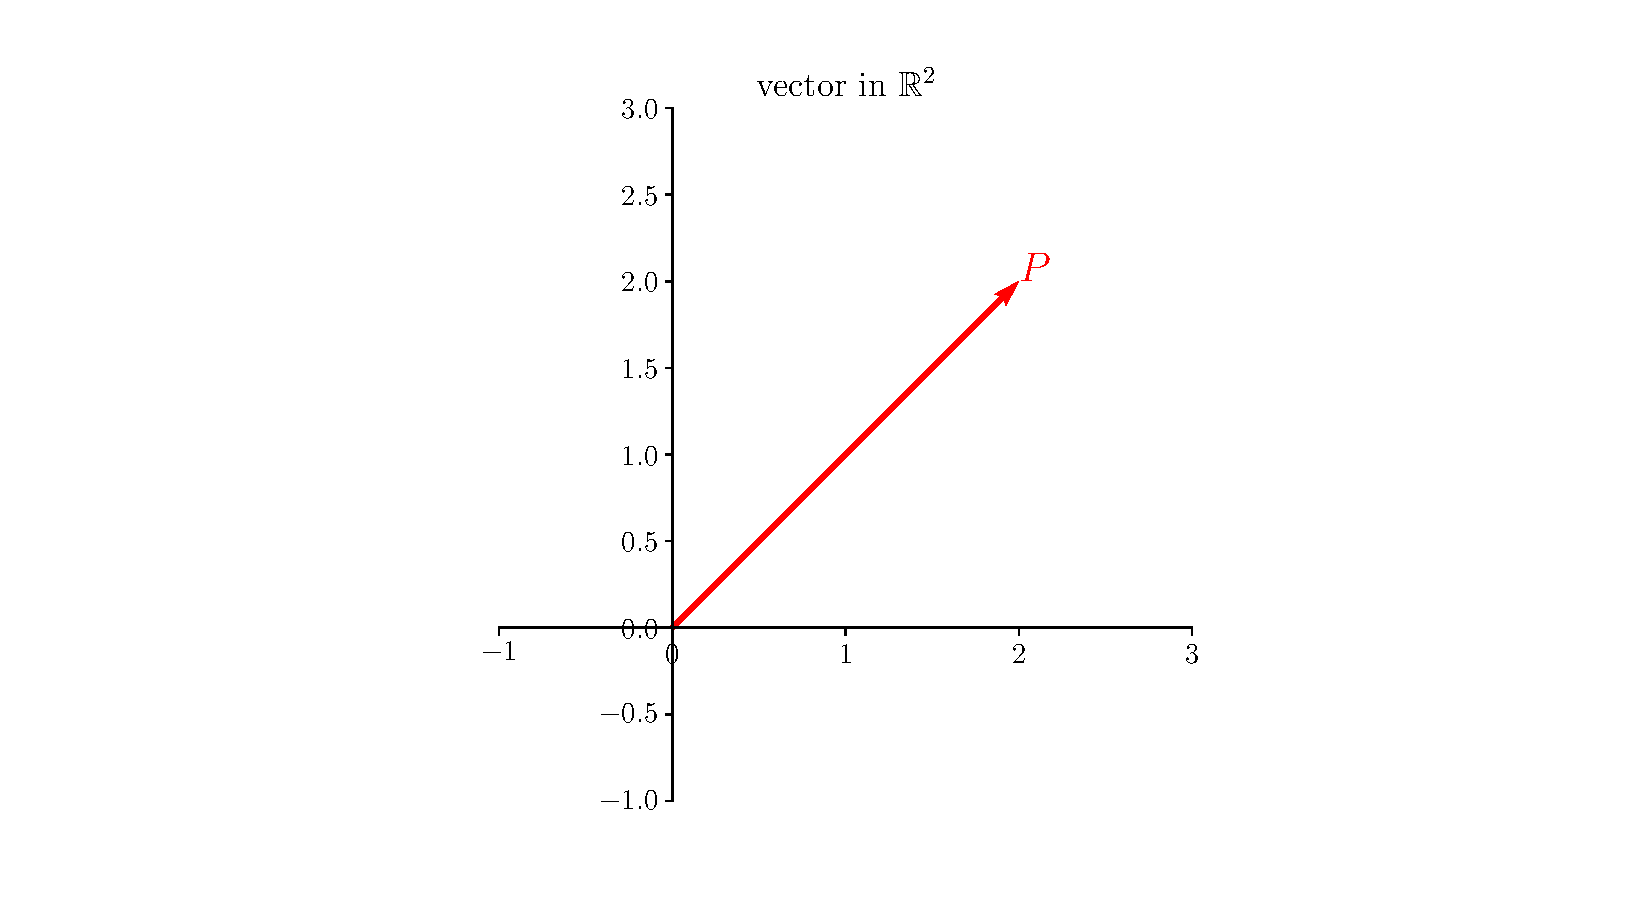
\includegraphics[width=0.5\textwidth]{eps/VectorInR2.eps}
			% \label{}命令为每个子图添加标签, 方便在正文中引用. 如果你不需要引用的话, 也可以不加这个命令, 写法在下面有: 
			% \label{}命令的{}内第一个{}中的内容fig:subfig1就是你插入的这张子图的标签, 注意每个标签都不能一样, 要用合适的编号去区分, 比如1, 2, 3......
			% \label{}命令中{}内\includegraphics[]{}就是真正插入图片的命令, []中的是图片的一些参数, {}就是图片的相对路径
			% width=0.4\textwidth 就是设置图片的大小, 这里设置的是文档宽度(\textwidth)的0.4倍, 在设置时注意不要超宽, 不然会报错, 大家多设置几个数尝试一下就能理解了
		}
		\subfloat[这两个向量是同一个,因为它们的大小和方向都一样]
		{
			\label{fig:same.vector}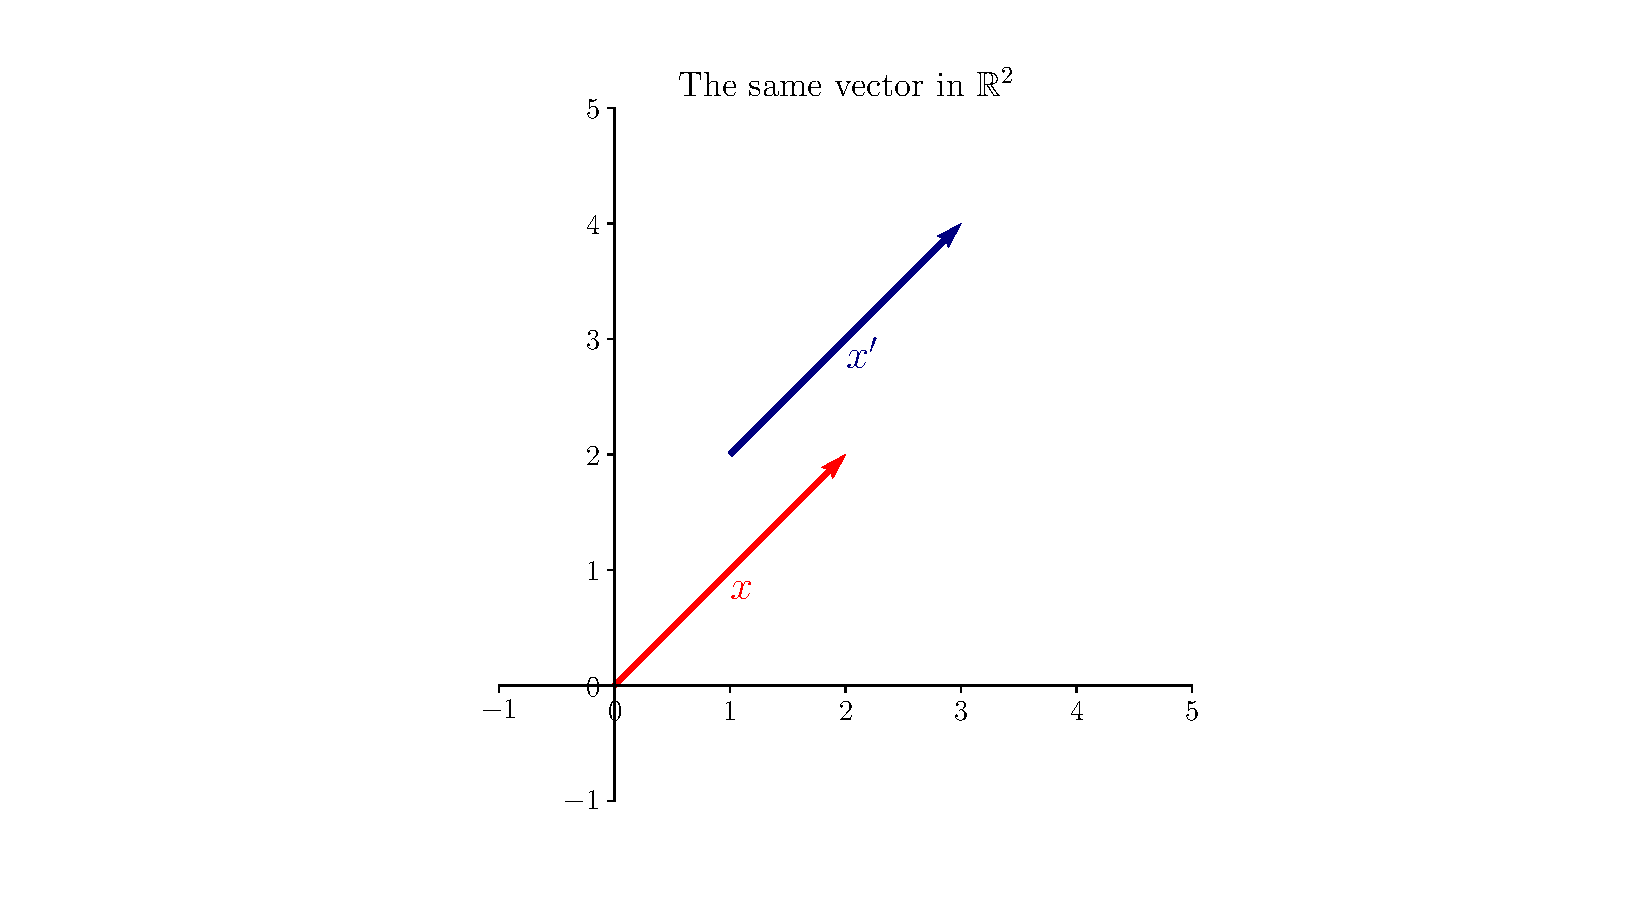
\includegraphics[width=0.5\textwidth]{eps/SameVectorInR2.eps}
		}
		\caption{二维向量}    % 整个图片的说明, 注释写在{}内
		\label{fig:intro.vector}            % 整个图片的标签编号, 注意这里跟子图是一样的道理, 标签不能重复 
\end{figure}

\section{向量的运算法则}
\label{sec:vector.operator}
\subsection{加法}

\begin{definition}{向量的加法}
	\label{def:vectoraddition}
	若$x,y\in \mathbb{F}^n,x=(x_1,x_2,x_3,\cdots,x_n),y=(y_1,y_2,y_3,\cdots,y_n)$则$x+y$定义为$$x+y:=(x_1+y_1,x_2+y_2,x_3+y_3,\cdots x_n+y_n)$$
\end{definition}

实际上两个向量相加,就是将它们元组里面的所有元素依次相加得到一个新的元组。

\begin{ascolorbox1}{思考}
	维度不同的向量是否可以相加?
\end{ascolorbox1}

要解答这个问题,我们需要返回到定义中,我们只定义了维度相同都为$n$的向量相加,并没有定义维度不同的向量相加的情况,所以这是一个未定义的行为;所以下面的对向量的运算均是在同一维度下进行。同理,向量与标量无法相加。

\begin{postulate}
	只有维度相同的向量才能互相相加。
\end{postulate}

同样,向量的加法也满足交换律:
\begin{corollary}
	若$x,y\in \mathbb{F}^n$,则$x+y=y+x$。
\end{corollary}

下面是简单的对此性质的证明(读者不作要求)。

\begin{proof}
	若$x,y\in \mathbb{F}^n,x=(x_1,x_2,x_3,\cdots,x_n),y=(y_1,y_2,y_3,\cdots,y_n)$则$$x+y=(x_1+y_1,x_2+y_2,x_3+y_3,\cdots x_n+y_n)$$根据标量加法的交换律可知
	\begin{equation*}
	x+y=(y_1+x_1,y_2+x_2,y_3+x_3,\cdots y_n+x_n)=y+x \teoe
	\end{equation*}
\end{proof}

如果我们将其反映在二维坐标系上,那应该是这样的
\begin{figure}[htbp]
	\centering
	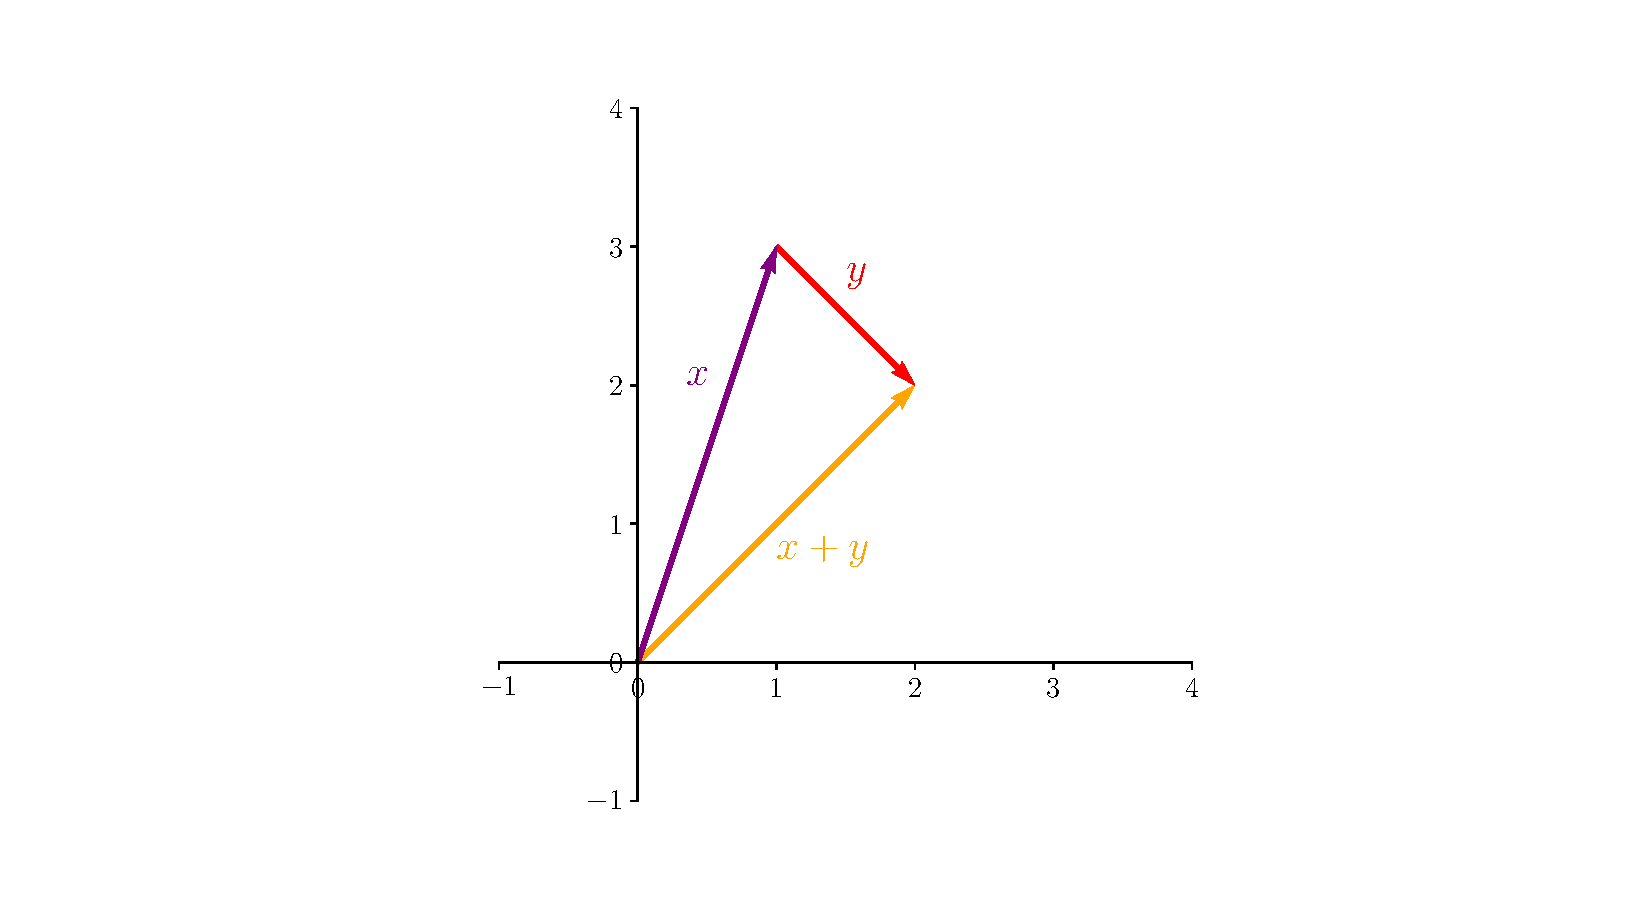
\includegraphics[width=0.7\linewidth]{eps/SumOf2Vectors}
	\caption{平面内两向量之和}
	\label{fig:sumof2vectors}
\end{figure}


\subsection{0 向量}

我们之前说过,向量与标量无法相加,所以在$\mathbb{F}^n$内我们定义$n$维0向量作为加法的单位元,即若$x,y\in \mathbb{F}^n$,$x+y=x$,那么$y$就是0 向量。

\begin{definition}{0 向量}
	若$\alpha,\beta \in \mathbb{F}^n$且$\alpha+\beta = \alpha$,那么$\beta$为空间$\mathbb{F}^n$的单位元,我们将其称为0向量,显然0向量就是一个全是由0组成的$n$元组,记作$\boldsymbol{0}$\footnote{实际上是以粗体形式出现的0},那么$$\boldsymbol{0}=(0,0,0,\cdots,0)$$
\end{definition}

\subsection{加法逆元}

类似于标量加法的$x,y\in \mathbb{C},x+y=0$,其中标量0表示标量加法的单位元,其中$y=-x$,那么在空间$\mathbb{F}^n$中同样表示若$\alpha,\beta \in \mathbb{F}^n,\alpha+\beta=\boldsymbol{0}$,$\beta=-\alpha$表示$\alpha$的加法逆元。

\begin{definition}{加法逆元}
	对于$\alpha \in \mathbb{F}^n$,$\alpha$的加法逆元表示满足下面条件的向量$-\alpha\in \mathbb{F}^n$有$$\alpha+(-\alpha)=\boldsymbol{0}$$换而言之当$\alpha=(a,b,c,d,\cdots)$时,$-\alpha=(-a,-b,-c,-d,\cdots)$
\end{definition}

\subsection{标量乘法}

\begin{definition}{向量的标量乘法}
	\label{def:facmul}
	若标量$\lambda \in \mathbb{F}$,其对一个向量$x=(x_1,x_2,x_3,\cdots,x_n)$的乘积满足以下的运算法则$$\lambda(x_1,x_2,x_3,\cdots,x_n):=(\lambda x_1,\lambda x_2,\lambda x_3,\cdots,\lambda x_n)$$
\end{definition}

实际上如图\ref{fig:mulfsn}所示,向量的标样乘法从$\mathbb{R}^2$的几何意义来看表示的是向量长度的缩放倍率。例如$x=(1,2)$那么$2x=(2,4)$.

\begin{figure}[htbp]
	\centering
	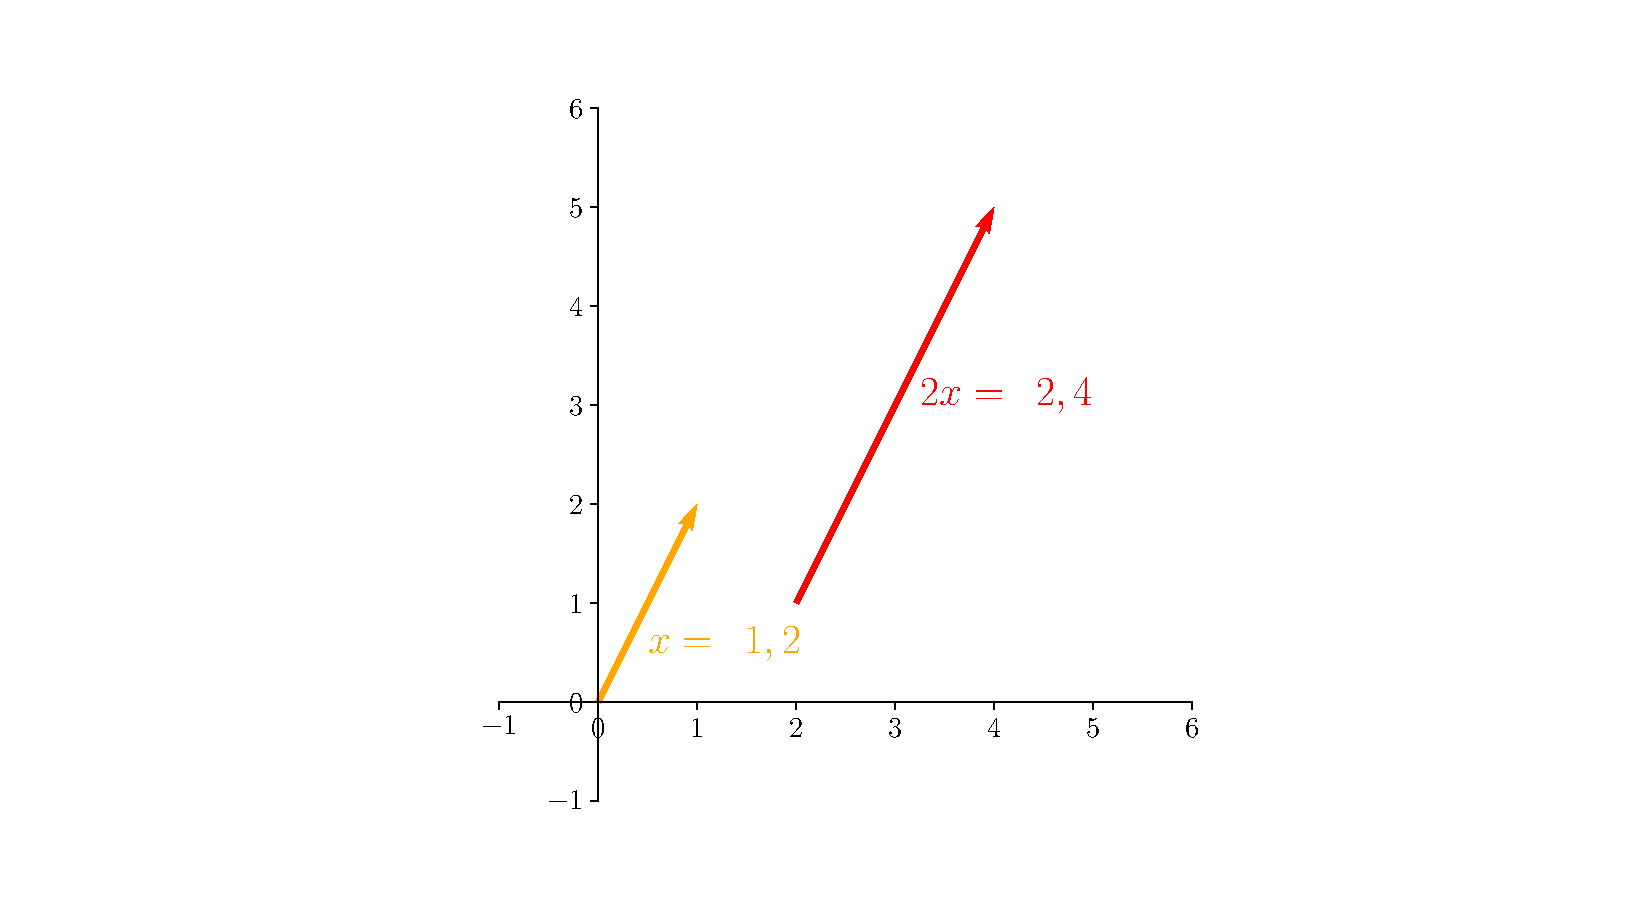
\includegraphics[width=0.7\linewidth]{figure/eps/MulFSn}
	\caption{向量长度的缩放倍率}
	\label{fig:mulfsn}
\end{figure}

同时,向量的标量乘法满足标量结合律。
\begin{corollary}
	若$a,b\in \mathbb{F},x\in \mathbb{F}^n$,满足$(ab)x=a(bx)$。
\end{corollary}

至此,我们对向量的运算法则做一个总结,我们目前只定义了2种运算法则,一种是向量和,另一种是标量积,下面我们会用这两种运算讲解一个特殊的集合,使得这个集合由这两部分构成。

\begin{example}
	已知$x\in \mathbb{R}^4$且满足$(1,1,4,-5)+2x=(5,1,-4,1)$,求$x$。
	\tcblower
	\textcolor{purple}{\textbf{解}}:等式两边同时加上$(1,1,4,-5)$的逆元$(-1,-1,-4,5)$可得$$2x+(0,0,0,0)=(5,1,-4,1)+(-1,-1,-4,5)=(4,0-8,6)$$设$x=(a,b,c,d)$可得$$(2a,2b,2c,2d)=(4,0,-8,6)$$由此可以得到方程组$$\left\{\begin{matrix} 
		2a=4 \\
		2b=0 \\
		2c=-8 \\
		2d=6
	\end{matrix}\right. $$所以可得$x=(2,0,-4,3)$
\end{example}

读者平时在作业的时候无需大费周章地严格用定理来写题目,如果你熟练的话可以直接自己写一个关于向量的减法法则(实际上就是加法法则的逆运算)来做题。

\section{线性空间$\mathbb{R}^2$与$\mathbb{R}^3$}
\subsection{线性空间}
\label{subsec:linearSpace}
如果要刻画线性空间,我们先从空间说起。

前文我们提到了``空间$\mathbb{F}^n$'',那么我们可以在此断章取义地说,空间就是一个集合,而线性空间是一个特殊的集合,我们给它一个符号$V$来表示。

下面给出定义来描述线性空间特殊的地方,线性空间$V$是一个带有加法和标量乘法的集合,下面我们将前面的向量的运算法则抽象化来定义它们。不过在此之前,我希望和大家来聊一聊一些你可能不是很了解的名词,例如函数(function)。
\begin{definition}{函数(一元)}
	对于任意的非空集合$A,B$,对集合$A$施加一个法则$f$使得$A$中的元素$x$可以转变为集合$B$中的元素$y$,记作$f(x)$或$f: A\rightarrow B$,即$y=f(x)$。
\end{definition}

上面讲述了函数的一般情形,那就是一元函数;一元函数有一个显著的特点,就是``输入一个元素并输出一个元素'',当然还有多元函数,下面请读者思考。

\begin{ascolorbox1}{思考}
	两个可以相加的元素进行加法运算,这是一种函数吗?
\end{ascolorbox1}

回答是肯定的,只不过这就不是一元函数了,这是二元函数,即``输入两个元素并输出一个元素'',翻译成数学的符号语言可以是:若$a,b\in A$则$f(a,b):=a+b$。同理,如果我们将集合内的元素特殊化为一种向量,那就是若$a,b\in \mathbb{F}^n$则$f(a,b):=a+b$。

那我们回到线性空间上来,如果一个集合$V$满足下面这一些条件的我们称其为线性空间\footnote{有些教材会叫做向量空间}。

\begin{definition}{线性空间上的加法与标量乘法}
	若集合$V$与数集$\mathbb{F}$满足以下的性质,则称$V$为$\mathbb{F}$上的线性空间:
	\begin{enumerate}
		\item $V$上的加法是一个函数使得任意一对$u,v \in V$经过法则$f(u,v)=u+v$转变为$V$中的另一个元素,这说明了$u+v\in V$。
		\item $V$上的标量乘法是一个函数使得任意一个$\alpha \in \mathbb{F}$和$u\in V$经过法则$f(u)=\alpha u$转变为$V$中的另一个元素,这说明了$\alpha u \in V$。
	\end{enumerate}
\end{definition}

根据的定义,线性空间$V$具有如下的性质:

\begin{definition}{线性空间的性质}
	\label{linear.space.sit}
	线性空间就是带有加法和标量乘法的集合$V$,满足如下的性质:
	\begin{itemize}
		\item 交换性(commutativity):对于所有的$u,v\in V$都有$u+v=v+u$;
		\item 结合性(associativity):对于所有的$u,v,w \in V$和$a,b\in \mathbb{F}$都有$(u+v)+w=u+(v+w)$和$(ab)v=a(bv)$;
		\item 加法单位元(additive identity):存在$\boldsymbol{0}\in V$使得对于所有的$v\in V$都有$v+\boldsymbol{0}=v$;
		\item 加法逆元(additive inverse):对于每一个$v\in V$都存在$w\in V$使得$v+w=\boldsymbol{0}$;
		\item 乘法单位元(multiplicative identity):对于所有的$v\in V$都存在$w\in V$使得$v+w=0$;
		\item 分配性质(distributive properties):对于所有的$a,b \in \mathbb{F}$和$u,v \in V$都有$a(u+v)=au+av$和$(a+b)v=av+bv$。
	\end{itemize}
\end{definition}

\begin{ascolorbox1}{思考}
	空集可以是线性空间吗?
\end{ascolorbox1}

答案为不是,因为空集$A$它不存在单位元$\boldsymbol{0}\in A$所以并不能是线性空间,此外,需要注意的是我们一般会说$V$是$\mathbb{F}$上的线性空间而不会直接说$V$是线性空间,因为我们在定义线性空间的时候,依赖了$\mathbb{F}$这个标量数集。

如之前所承诺的,下面给出向量的定义。

\begin{definition}{向量}
	线性空间中的元素称为向量。
\end{definition}

读者可能会觉得这样给出会有些突然,我们不妨反过来看看向量作为线性空间$V$的元素,是否满足定义\ref{linear.space.sit}的6个条件,然后与读者高中所学的向量的特性对比,发现是否吻合。如果读者觉得这样做还是太抽象,我们不妨研究一下在线性空间$\mathbb{R}^2$与$\mathbb{R}^3$中向量的相关图形表现。

\subsection{直线,平面与三维空间上的向量}

向量同时具有长度和方向两种特性,如果我们在$\mathbb{R}^2$上绘制平面直角坐标系来图像化向量这一个概念的话,向量就是一个有向箭头,由起点和终点构成,若一个有向箭头的起点为$P$,终点为$Q$,我们将此有向箭头\footnote{向量与有向箭头的区别在于,长度相同且方向相同的有向箭头,可以有很多个表示,如图\ref{fig:same.vector}所示,而这两个有向箭头表示的向量是同一个。不过,通常而言,该有向线段也可直接称为向量}记为$\overrightarrow{PQ}$。若$a\in \mathbb{R}^2,a=\overrightarrow{PQ}$,则向量$a$的长度为线段$PQ$的长度,记作$\left \| a \right \| $。

\begin{definition}{$\mathbb{R}^2$上向量的长度}
	\label{def:lengthOfVec}
	若$x\in \mathbb{R}^2$且$x=(x_1,x_2)$,则$x$的长度$\left \| x \right \| $为$$\left \| x \right \| := \sqrt{x_1^2+x_2^2}$$
\end{definition}

\begin{example}
	已知$a,b\in \mathbb{R}^2$,点$O$为平面直角坐标系的原点,$P_1,P_2$分别为一条线段的两个端点,$M$为该线段的重点,其中$a=\overrightarrow{OP_1},b=\overrightarrow{OP_2}$,求$\overrightarrow{OM}$。
	\tcblower
	\textcolor{purple}{\textbf{解}}:在长度上$\left \| \overrightarrow{P_1M} \right \|=\left \| \overrightarrow{MP_2} \right \|$且在同一条直线上,所以$\overrightarrow{P_1M}=\overrightarrow{MP_2}$,根据向量的加法法则有$$\overrightarrow{OM}=\overrightarrow{OP_1}+\overrightarrow{P_1M},\overrightarrow{OM}=\overrightarrow{OP_2}-\overrightarrow{P_1M}$$前后两式相加可得$$\overrightarrow{OM}=\frac{a+b}{2}$$
\end{example}

此外由于向量具有方向性,且可以随处移动,由此我们也可以由此性质确定$\mathbb{R}^2$和$\mathbb{R}^3$空间中直线的方向并确定直线的方程。

\begin{definition}{直线的方向向量}
	空间直线的方向用一个与该直线平行的有向箭头表示,该有向箭头所表示的向量即为空间直线的方向向量。
\end{definition}

\begin{figure}[htbp]
	\centering
	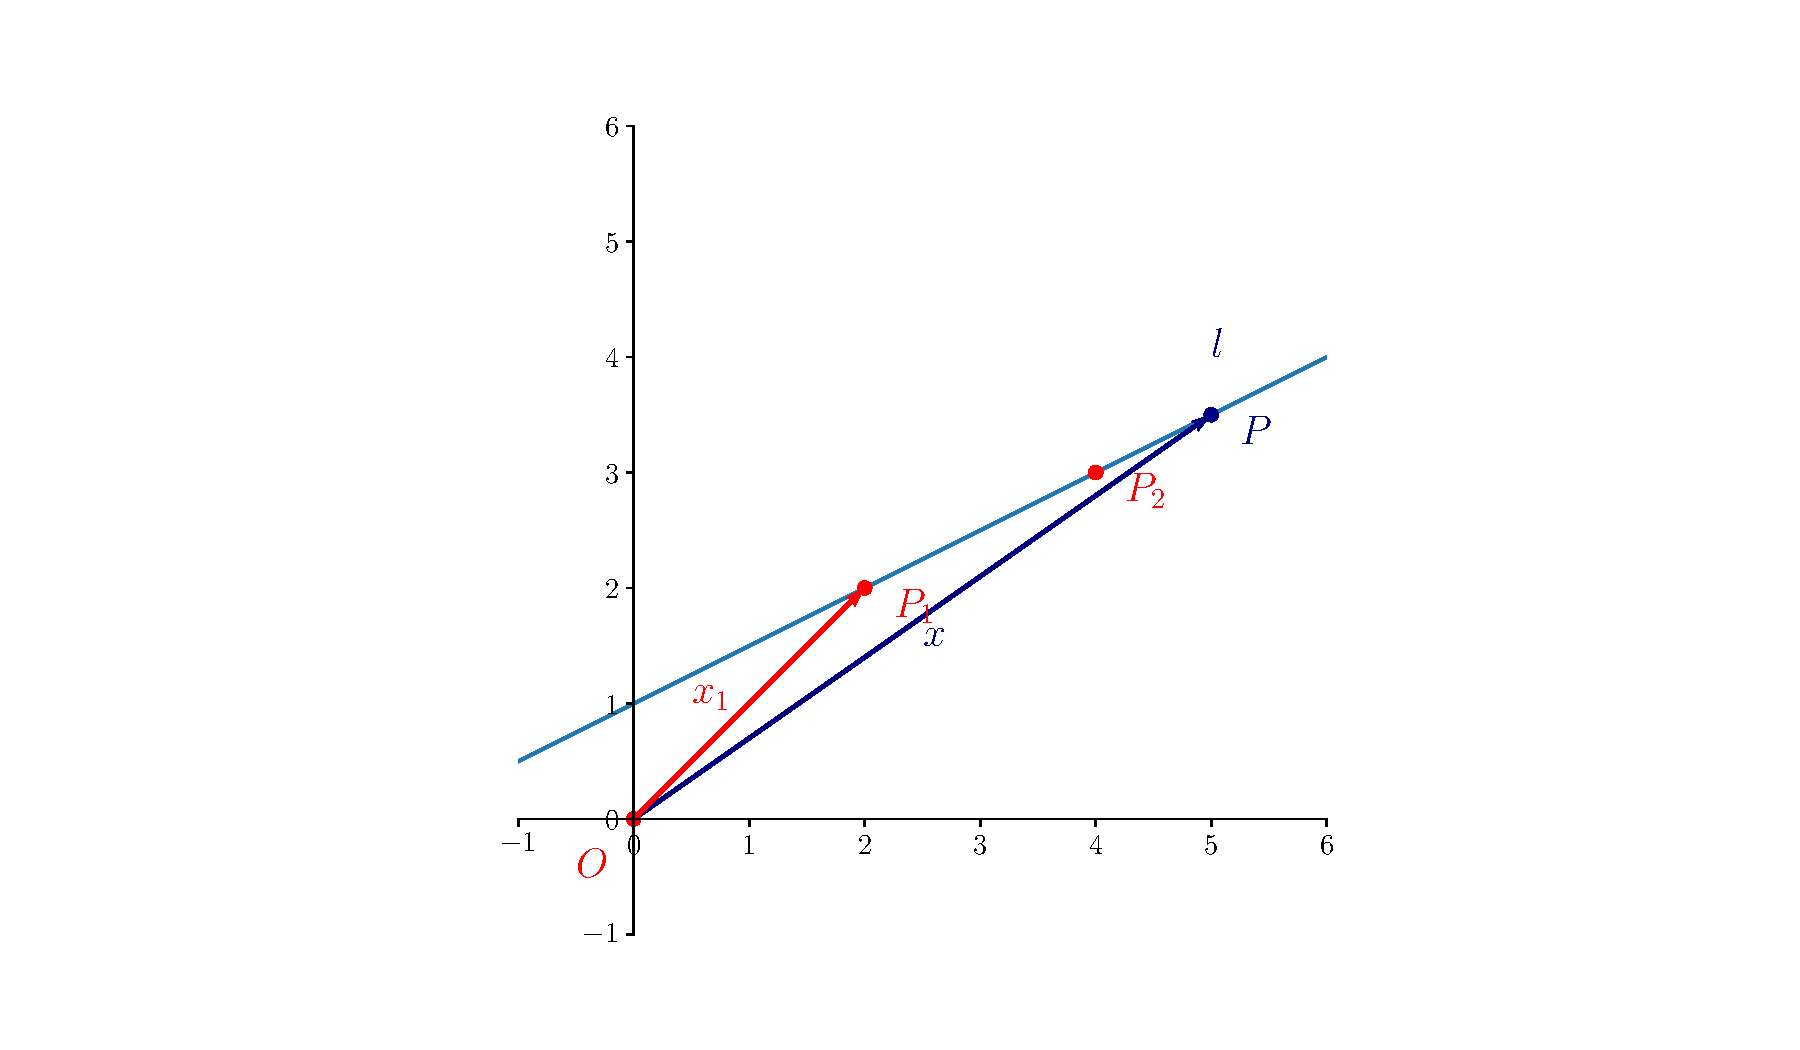
\includegraphics[width=0.7\linewidth]{figure/eps/LineAndVector2d}
	\caption{方向向量与直线方程}
	\label{fig:lineandvector2d}
\end{figure}

如图\ref{fig:lineandvector2d}所示,$P_1$和$P_2$都在直线$l$上,设$x,x_1\in \mathbb{R}^2,x=\overrightarrow{OP},x_1=\overrightarrow{OP_1}$,有向箭头$\overrightarrow{P_1P_2}$在直线$l$上,若向量$a\in \mathbb{R}^2$满足$a=\overrightarrow{P_1P_2}$,则该向量$a$是这条直线的方向向量。

既然知道了直线的方向向量和$O$到直线上某一点的有向箭头所表示的向量,我们就可以建立一个等式来唯一确定一条直线,设$t\in \mathbb{R}$,那么对于任意处于直线上的$P$点,总存在$t$使得$x=\overrightarrow{OP}$满足$$x=x_1+ta$$如果我们设直线上的$P$点坐标为$(x,y)$那么$x=(x,y)$设$P_1$的坐标是$(x_1,y_1)$,$P_2$的坐标是$(x_2,y_2)$,于是乎$a=(x_2-x_1,y_2-y_1)$,由$x=x_1+ta$并代入坐标,根据向量的加法与标量乘积的运算定理,我们可以得到下面的式子$$\left\{\begin{matrix} 
	x-x_1=t(x_2-x_1) \\  
	y-y_1=t(y_2-y_1)
\end{matrix}\right. $$所以我们可以得到这就是经过$P_1$和$P_2$两点的参数方程,如果要进一步往下化简的话,我们可以得到$$\frac{x-x_1}{x_2-x_1}=\frac{y-y_1}{y_2-y_1}$$

\begin{example}
	求二维空间$\mathbb{R}^2$内直线方程$3x+4y-5=0$的一个方向向量。
	\tcblower
	\textcolor{purple}{\textbf{解}}:设$P_1,P_2$点坐标分别为$(x_1,y_1),(x_2,y_2)$,则$a\in \mathbb{R}^2,a=\overrightarrow{P_1P_2}$为其一个方向向量,令$x_1=0$则$\displaystyle y_1=\frac{5}{4}$,$\displaystyle \overrightarrow{OP_1}=\left( 0,\frac{5}{4} \right)$,令$y_2=0$则$\displaystyle x_2=\frac{5}{3}$,$\displaystyle \overrightarrow{OP_2}=\left(\frac{5}{3},0\right)$,$\overrightarrow{P_1P_2}=\overrightarrow{OP_2}-\overrightarrow{OP_1}$所以该直线的一个方向向量为$\displaystyle \left( \frac{5}{3},-\frac{5}{4} \right) $
\end{example}

接下来我们将维度扩展到三维空间$\mathbb{R}^3$内,依然有$$x=x_1+ta$$由此如果$P_1$与$P_2$的坐标分别为$(x_1,y_1,z_1)$和$(x_2,y_2,z_2)$,我们将会得到下面的等式$$\frac{x-x_1}{x_2-x_1}=\frac{y-y_1}{y_2-y_1}=\frac{z-z_1}{z_2-z_1}$$这就是空间内的直线方程(实际上就是两个一次方程)

\begin{example}
	求三维空间$\mathbb{R}^3$内直线方程$$\left\{\begin{matrix} 
		x+y+z=3 \\  
		x+2y+3z=6
	\end{matrix}\right. $$的一个方向向量。
	\tcblower
	\textcolor{purple}{\textbf{解}}:设$P_1,P_2$点坐标分别为$(x_1,y_1,z_1),(x_2,y_2,z_2)$,则$a\in \mathbb{R}^3,a=\overrightarrow{P_1P_2}$为其一个方向向量,令$x_1=1$则$\displaystyle y_1=1,z_1=1$,$\displaystyle \overrightarrow{OP_1}=\left( 1,1,1 \right)$,令$x_2=0$则$\displaystyle y_2=3,z_2=0$,$\displaystyle \overrightarrow{OP_2}=\left(0,3,0\right)$,$\overrightarrow{P_1P_2}=\overrightarrow{OP_2}-\overrightarrow{OP_1}$所以该直线的一个方向向量为$\displaystyle \left( -1,2,-1 \right) $
\end{example}

同样的,根据两条相交直线可以确定平面,如果我们使用向量来考虑$\mathbb{R}^3$上的平面的话,通过两个不互相平行的非零向量和一点也能确定一个平面,如图\ref{tikz:space.face}所示。

\begin{figure}[htbp]
	\centering
	\tdplotsetmaincoords{60}{70}

\begin{tikzpicture}[yscale=1.5,xscale=1.5,line width=0.8pt,tdplot_main_coords]
	\coordinate (A) at (0,0,0);
	\coordinate (B) at (4,0,0);
	\coordinate (C) at (4,3,0);
	\coordinate (D) at (0,3,0);
	\coordinate (O) at (0.5,0.5,2);
	
	\coordinate (P) at (3.5,2.5,0);
	\coordinate (P1) at (0.5,0.5,0);
	\coordinate (P2) at (2.5,0.5,0);
	\coordinate (P3) at (0.5,2,0);
	\coordinate (P3t) at (0.5,2.5,0);
	\coordinate (P2t) at (3.5,0.5,0);
	
	
	\draw[rounded corners=0.05pt](A)--(B)--(C)--(D)--(A);
	
	\draw[->,>=Stealth](O)node[above=3.5pt,right=3pt]{$O$}--(P)node[above=2.5pt,right=2.5pt]{$P$};
	\draw[->,>=Stealth](O)--(P1)node[above=2.5pt,left=1.5pt]{$P_1$};
	\draw[->,>=Stealth](P1)--(P2)node[above=2.5pt,right=2.5pt]{$P_2$};
	\draw[->,>=Stealth](P1)--(P3)node[right=2.5pt]{$P_3$};
	\draw[dashed](P1)--(P3t)--(P)--(P2t)--(P1);
	\draw[->,>=Stealth](P1)--(P);
	%\draw(P)node[above=3.5pt,right=3pt]{$P$};
\end{tikzpicture}
	\caption{$P$在平面上}
	\label{tikz:space.face}
\end{figure}

类比于直线的向量表示,设向量$x,x_1,a,b\in \mathbb{R}^3$,$P,P_1,P_2,P_3$点在平面上,令$x=\overrightarrow{OP},a=\overrightarrow{P_1P_2},b=\overrightarrow{P_1P_3},x_1=\overrightarrow{OP_1}$,设$t,s\in \mathbb{R}$,对于任意处于平面上的$P$点,总存在$t,s$使得$x=\overrightarrow{OP}$满足$$x=x_1+ta+sb$$由于过空间内不在同一直线上的三个点写方程很复杂,限于篇幅结构笔者不再详细介绍推导过程\footnote{可能会有读者会说平面的点法式方程,我知道学霸读者很多,但是笔者需要考虑给入门的选手讲清楚这些,后面我们会慢慢接触它们,请不要着急。}。不过笔者在此给出平面方程的一般形式(只有一个等式)。$$ax+by+cz+d=0,a,b,c,d\in \mathbb{R}$$

\subsection{其他线性空间}

上面我们讲了$\mathbb{R}^2$和$\mathbb{R}^3$是一种线性空间,更一般的例子就是$\mathbb{R}^n$,再一般的例子就是$\mathbb{C}^n$。

\begin{definition}{实线性空间与复线性空间}
	\begin{itemize}
		\item $\mathbb{R}$ 上的线性空间称作实线性空间。
		\item $\mathbb{C}$ 上的线性空间称作复线性空间。
	\end{itemize}
\end{definition}

除此之外,还有多项式空间也是线性空间,下面给出定义。

\begin{definition}
	所有次数不超过$n$的实系数多项式的集合,记作$P_n$。
\end{definition}

$P_n$ 中的元素是形如 $p(x) = a_0 + a_1 x + a_2 x^2 + \cdots + a_n x^n$ 的多项式,其中 $a_0, a_1, \dots, a_n \in \mathbb{R}$,接下来我们来验证$P_n$是线性空间。

\begin{corollary}
	$P_n$是$\mathbb{R}$或$\mathbb{C}$上线性空间。
\end{corollary}

下面给出证明(读者并不要求)

\begin{proof}
	验证加法,两个多项式相加是按系数相加,例如:$$p(x) + q(x) = (a_0 + b_0) + (a_1 + b_1)x + \cdots + (a_n + b_n)x^n$$可以得到他们的和依然是多项式。其次验证标量乘法,标量 $c \in \mathbb{R}$ 与多项式 $p(x)$ 的乘积是$$c p(x) = c a_0 + c a_1 x + \cdots + c a_n x^n$$所得的结果依然是多项式,若$P(x)=0$,代表的是该线性空间的零向量,满足线性空间的所有公理。$\square$
\end{proof}

\begin{ascolorbox1}{思考}
	你能不能举出其他的一些例子表示线性空间?
\end{ascolorbox1}

\section{子空间}

\subsection{子空间(subspace)的定义}

\begin{definition}
	如果$V$的子集$U$也是线性空间,则称$U$是$V$的子空间。
\end{definition}

例如$U=\left\{ (x_1,x_2,0) \mid x_1,x_2 \in \mathbb{R} \right\}$是$\mathbb{R}^3$的子空间。需要要注意的是,线性空间的子集也得是线性空间所以才能是子空间,所以请读者思考下面的一个问题。

\begin{ascolorbox1}{思考}
	$U=\left\{ (x_1,x_2,1) \mid x_1,x_2 \in \mathbb{R} \right\}$是否是$\mathbb{R}^3$的子空间?
\end{ascolorbox1}

答案为不是,因为它不满足$\boldsymbol{0}\in U$,根本就不是线性空间,所以不是$\mathbb{R}^3$的子空间。除此之外,子空间需要满足下面的情况(也就是说,也需要满足作为线性空间的条件)。

\begin{corollary}
	当且仅当 $V$ 的子集 $U$ 满足以下三个条件时,$U$ 是 $V$ 的子空间。
	\begin{itemize}
		\item 存在加法单位元$\boldsymbol{0}\in U$;
		\item 对于加法封闭,即$v,w\in U$满足$v+w\in U$;
		\item 对于标量乘法封闭,即$\lambda \in \mathbb{F},v\in U$满足$\lambda v\in \mathbb{F}$。
	\end{itemize}
\end{corollary}

\begin{ascolorbox1}{思考}
	若集合$U=\left\{ (x_1,x_2,0) \mid x_1,x_2 \in \mathbb{R} \right\}$,集合$T=\left\{ (0,0,x_3) \mid x_3 \in \mathbb{R} \right\}$,$T\cup U$是否是$\mathbb{R}^3$的子空间?
\end{ascolorbox1}

答案为不是,因为它不满足对于加法封闭,取$u\in U,u=(1,1,0),t \in T,t=(0,0,1)$,$u+t=(1,1,1) \notin U\cup T$,所以不是$\mathbb{R}^3$的子空间。

\subsection{子空间之和}

为了更深入了解线性空间以及知识完整性,下面讲解子空间和的概念。

\begin{definition}{子空间的和}
	子空间的和是有其所有元素可能的和所构成的集合,其结果仍是子空间。若$V_1,V_2,V_3,\cdots,V_m$是$V$的子空间,则子空间的和$V_s$记作$$V_s=V_1+V_2+V_3+\cdots+V_m=\sum_{i=1}^{m}V_i $$或者说来$$V_s=\sum_{i=1}^{m}V_i =\left\{ \sum_{i=1}^{m}v_i \mid i\in \mathbb{N}^+,v_i \in V_i \right\}$$
\end{definition}

不要被定义上的Sigma符号吓跑了,实际上就是分别任意两个属于不同子空间的元素相加后的新元素所构成的空间,例如子空间$V_1=\left\{ (x_1,x_2,0)\mid x_1,x_2\in \mathbb{R} \right\}$和$V_2=\left\{ (0,x_3,x_4)\mid x_3,x_4\in \mathbb{R} \right\}$,则$V_1,V_2$子空间的和是$\mathbb{R}^3$,即$\mathbb{R}^3$中所有的元素$r$均存在$t,s\in \mathbb{R}$使得$v_1\in V_1$,$v_2\in V_2$满足$$r=tv_1+sv_2$$

所以可以记作$\mathbb{R}^3=V_1+V_2$。

上面讲了子空间的和,请读者先思考子空间的和与子空间的并的区别。

\begin{ascolorbox1}{思考}
	子空间的并是否一定是子空间?在什么情况下子空间的并是子空间?
\end{ascolorbox1}

首先回答第一个,子空间的并不一定是子空间,如上面的一个思考$T\cup U$一样,$U,T$均为$\mathbb{R}^3$的子空间,但是我们证明了它们的并集不是子空间。对于第二个问题,首先我们考虑$V$子空间$T$和$U$,如果$T$是$U$的非空子集(思考为什么非空?),那么$T \cup U=U$是子空间显然成立,若$T$不是$U$的非空子集,设$t\in T,u\in U$由子空间的性质应有$t+u$属于$V$,即$t+u$可能属于$T$也可能属于$U$。但是若$t+u$属于$T$,而根据封闭性$u=(t+u)-t$也应当属于$T$,$t+u$和$u$都是子空间$T$的元素,所以与``若$T$不是$U$的非空子集''的设定不符。

\begin{corollary}
	两个子空间的并集是子空间,当且仅当其中一个包含于另一个。
\end{corollary}

\subsection{直和}

首先我们回顾一下笛卡尔积\footnote{笛卡尔积的另一个名称叫做直积,和本部分的直和的运算方式有关联。},如果读者已经忘记了的话请阅读定义\ref{def:dicar},我们了解到$\mathbb{R}^3$空间由$\mathbb{R}\times\mathbb{R}\times\mathbb{R}$通过笛卡尔积生成。而直和也是生成生成空间的一种方式,是一种特殊的子空间之和。

\begin{definition}{直和(direct sum)}
	设$V_1,V_2,V_3,\cdots,V_m$是$V$的子空间,如果$V_1+V_2+V_3+\cdots+V_3$中的每个元素都能用$\sum_{i=1}^{m}v_i ,v_i\in V_i$唯一地表示出来,则称子空间之和$\sum_{i=1}^{m}V_i $为直和,可写作$$V=V_1\oplus V_2\oplus V_3\oplus \cdots \oplus V_m$$
\end{definition}

例如$A=\left\{ (x,y,0)\mid x,y \in \mathbb{R} \right\},B=\left\{ (0,0,z)\mid z\in \mathbb{R} \right\}$,则$\mathbb{R}^3=A \oplus B$;而$A=\left\{ (x,y,z)\mid x,y,z \in \mathbb{R} \right\},B=\left\{ (0,0,z)\mid z\in \mathbb{R} \right\}$,则$\mathbb{R}^3\neq A \oplus B$。

\begin{corollary}
	$U$ 和 $W$ 是 $V$ 的子空间且$V=U\oplus W$,当且仅当$W\cap U=\left\{ 0 \right\}$。
\end{corollary}

接下来我们继续研究构建线性代数的基本内容,即向量与空间的关系。

\section{张成空间与线性相关性}

\subsection{线性组合与张成空间}

一组向量进行标量乘法后相加形成的一个向量,称作该向量的线性组合。

\begin{definition}{线性组合(linear combination)}
	给定向量集合 $\{v_1, v_2, \dots, v_k\}$ 和标量集合 $\{c_1, c_2, \dots, c_k\}$,向量 $v$ 的线性组合表示为:$$v = c_1 v_1 + c_2 v_2 + \dots + c_k v_k$$其中,$c_1, c_2, \dots, c_k$ 称为组合系数。
\end{definition}

通过一组向量的线性组合所产生的向量能表示的空间是这个向量的张成空间,下面给出定义。

\begin{definition}{张成空间(span)}
	给定向量集合 $ S = \{v_1, v_2, \dots, v_k\} $(其中 $ v_i $ 是线性空间 $ V $ 中的向量),这些向量的张成空间是所有可能的线性组合构成的集合,记作:$$\text{Span}(S) = \{ c_1 v_1 + c_2 v_2 + \dots + c_k v_k \mid c_1, c_2, \dots, c_k \in \mathbb{F} \}$$如果$V=\text{Span}(S)$,则称向量集合$S$张成\footnote{这里的张成是动词。}空间$V$。
\end{definition}

例如$(1,2,4) \in \text{Span}(\left\{ (1,0,0),(0,1,2) \right\})$因为存在线性组合使得$(1,2,4)=(1,0,0)+2(0,1,2)$,而$(1,2,5) \notin \text{Span}(\left\{ (1,0,0),(0,1,2) \right\})$因为不存在线性组合使得$(1,2,5)=\lambda (1,0,0)+\beta (0,1,2)$。

再有例子$\mathbb{R}^3=\text{Span}(\left\{ (1,0,0),(0,1,0),(0,0,1) \right\})$,因为任何一个$v\in \mathbb{R}^3$都可以由$\left\{ (1,0,0),(0,1,0),(0,0,1) \right\}$的线性组合构成。

\begin{corollary}
	张成空间$\text{Span}(S)$是包含向量$S$空间的子空间。
\end{corollary}

不要笑!可能这个概念对读者来说就像$2+2=4$一样简单,这个推论是显然的,张成空间是子空间,但是我们还是来证明它。

\begin{proof}
	对于$V=\text{Span}(S),S=\left\{ v_1,v_2,v_3,\cdots,v_n \right\}$,有加法单位元$\boldsymbol{0}\in V$,在此空间$V$中$$\boldsymbol{0}=\sum_{i=1}^{n}(0v_i) $$在空间$V$中满足在加法封闭$$\sum_{i=1}^{n}a_iv_i+ \sum_{i=1}^{n}c_iv_i=\sum_{i=1}^{n}(a_i+c_i)v_i$$也满足在标量乘法下封闭$$\lambda \sum_{i=1}^{n}a_iv_i= \sum_{i=1}^{n}\lambda a_iv_i$$所以张成空间$\text{Span}(S)$是包含向量$S$空间的子空间。$\square$
\end{proof}

\subsection{线性相关性}

下面我们给出线性代数的一个关键定义,从此往后,我们线性代数研究的内容就是有限维的线性空间。

\begin{definition}{有限维线性空间}
	线性空间如果可以由其空间内的有限个向量张成,则这个线性空间是有限维的。
\end{definition}

同时,我们在此基础上研究线性相关性;设$v_1,v_2,v_3,\cdots,v_n \in V$且$v \in \text{Span}(V)$,根据张成空间的定义我们有$a_1,a_2,a_3,\cdots,a_n \in \mathbb{F}$使得$$v = \sum_{i=1}^{n}a_iv_i =a_1v_1+a_2v_2+a_3v_3+\cdots+a_nv_n$$若$v=\boldsymbol{0}$,我们有一组显然的结果,即当$a_1=a_2=a_3=\cdots=a_n=0$的时候,$v=\boldsymbol{0}$,然而通常来说,我们可能还会遇到其他的$a_i$组合也可以使得$v=\boldsymbol{0}$,于是我们做出如下定义:

\begin{definition}{线性无关\footnote{有些书中会写成线性独立}(linearly independent)}
	对于向量$v_1,v_2,v_3,\cdots,v_n$如果使得其线性组合$a_1v_1+a_2v_2+a_3v_3+\cdots+a_nv_n=\boldsymbol{0}$的情况只有$a_1=a_2=a_3=\cdots=a_n=0$,则称向量$v_1,v_2,v_3,\cdots,v_n$线性无关。
\end{definition}

\begin{definition}{线性相关(linearly dependent)}
	若一些向量不是线性无关的,就称为线性相关。
\end{definition}

给出例子,向量$(1,0,0),(2,0,0),(0,0,3)$是线性相关的,因为存在$\boldsymbol{0}=2(1,0,0)+(-1)(2,0,0)+0(0,0,3)$而$(1,0,0),(0,2,0),(0,0,3)$是线性无关的,因为只有$a_1=a_2=a_3=0$使得$\boldsymbol{0}=0(1,0,0)+0(0,2,0)+0(0,0,3)$。

\begin{example}
	向量$(2,3,1),(1,-1,2),(7,3,c)$线性相关,求$c$的值。
	\tcblower
	\textcolor{purple}{\textbf{解}}:若三个向量线性相关,则有$\alpha,\beta,\gamma \in \mathbb{R},\alpha (2,3,1)+\beta (1,-1,2)+\gamma (7,3,c)=0$,可得线性方程$$\left\{\begin{matrix} 
		2\alpha +1\beta+7\gamma = 0 \\  
		3\alpha +(-1)\beta+3\gamma=0 \\
		1\alpha +2\beta+c\gamma=0
	  \end{matrix}\right.$$若使得线性方程组有非全为0解,我们任意取$\alpha = 1$,则根据前两个式子可得$$\left\{\begin{matrix} 
		1\beta+7\gamma = -2 \\
		(-1)\beta+3\gamma= -3 
		\end{matrix}\right.$$解其可得$\beta=1.5,\gamma=-0.5$而$\alpha=1$,带入第三式,$1+2\times 1.5-0.5c=0$最终结果为$$c=8$$
\end{example}

\begin{corollary}
	如果一组向量线性相关,那么其中一个向量均可以由其他向量的线性组合表示。
\end{corollary}

\begin{proof}
	一组向量 $v_1, v_2, \dots, v_n$ 是线性相关的,当且仅当存在不全为零的标量 $c_1, c_2, \dots, c_n$,使得:$$c_1 v_1 + c_2 v_2 + \dots + c_n v_n = \mathbf{0}$$由于向量组线性相关,至少存在一个标量 $c_k \neq 0$($1 \leq k \leq n$)而将上述等式中的 $v_k$ 单独移到等式一侧:$$c_k v_k = -c_1 v_1 - c_2 v_2 - \dots - c_{k-1} v_{k-1} - c_{k+1} v_{k+1} - \dots - c_n v_n$$两边同除$c_k$可得$$v_k = -\frac{c_1}{c_k} v_1 - \frac{c_2}{c_k} v_2 - \dots - \frac{c_{k-1}}{c_k} v_{k-1} - \frac{c_{k+1}}{c_k} v_{k+1} - \dots - \frac{c_n}{c_k} v_n$$本题得证。$\square$
\end{proof}

这个例子也说明了线性相关的向量集合张成的空间与其去掉任意一个向量后张成的空间是同一个空间。

此外也有一条重要的结论,若向量集合$V$内的元素线性无关,则$V$中元素的个数不大于张成该空间$U$的向量的个数。举个例子,$\left( 0,0,1 \right)$和$(0,1,0)$在$\mathbb{R}^3$线性无关,而张成$\mathbb{R}^3$的向量可能由$(1,0,0),(0,1,0),(0,0,1)$(或更多其他3个不共面的向量)构成,但是既要线性无关,而且还要张成这个空间的向量集合(下面会给这些向量集合一个名字叫做基)在$\mathbb{R}^3$上为3个\footnote{关于这个推论可能会比较抽象,读者可以回想在高中的学习生活中,通过空间直角坐标系的三个基底可以表示整个空间,缺一不可,且3个不共面的向量都可以成为基底}。

\subsection{基与维数}

通过线性无关和张成空间的两个概念的结合,我们可以得到基的概念。

\begin{definition}{基(basis)}
	若$V$中的一组向量线性无关且能够张成$V$,则称这组向量的集合称作$V$的基。
\end{definition}

所以按照上面的定义,基有两个方面的约束:
\begin{itemize}
	\item 基的选取必须是线性无关的,例如$\left\{ (1,0),(2,0),(0,1) \right\}$不能选为$\mathbb{R}^2$的基,因为$\boldsymbol{0}=-2(1,0)+(2,0)+0(0,1)$,这个例子说明二维平面内的基不能共线。
	\item 基的选取必须能张成选取的空间,例如$\left\{ (1,0,0),(0,1,0) \right\}$不能选为$\mathbb{R}^3$的基,因为它们只能张成\\$\left\{ (x,y,0)\mid x,y \in \mathbb{R} \right\}$,这个例子说明两个不共线的向量只能表示整个平面。
\end{itemize}

集合$\left\{ (1,0,0,\cdots,0),(0,1,0,\cdots,0),(0,0,1,\cdots,0),\cdots,(0,0,0,\cdots,1) \right\}$是$\mathbb{F}^n$的基,它比较特殊,是为$\mathbb{F}^n$的\textbf{标准基}。

\begin{corollary}
	若空间$V$包含向量集合$S=\left\{ v_1,v_2,v_3,\cdots,v_n \right\}$且$S$是空间$V$的基,则仅有唯一的$a_1,a_2,a_3,\cdots \in \mathbb{F}$线性组合表示任意一个$V$的元素$v$,即每个$v\in V$都能唯一地表示成下面的形式:$$v=a_1v_1+a_2v_2+a_3v_3+\cdots+a_nv_n$$
\end{corollary}

\begin{example}
	求$U=\left\{ (a,b,c,d,e)\in \mathbb{R}^5 \mid a=2b,c=4d \right\}$的一个基集合。
	\tcblower
	\textcolor{purple}{\textbf{解}}:子空间 $ U $ 中的向量可以表示为:$$(a, b, c, d, e) = (2b, b, 4d, d, e)$$将向量表示为自由变量的线性组合$$(2b, b, 4d, d, e) = b(2, 1, 0, 0, 0) + d(0, 0, 4, 1, 0) + e(0, 0, 0, 0, 1)$$这表明 $ U $ 中的任意向量都可以由向量组 $ \left\{ (2, 1, 0, 0, 0), (0, 0, 4, 1, 0), (0, 0, 0, 0, 1) \right\} $ 线性表示,因此,子空间 $ U $ 的一个基集合为$$\left\{ (2,1,0,0,0), (0,0,4,1,0), (0,0,0,0,1) \right\}$$
\end{example}

接下来我们引入维数的概念:

\begin{definition}{维数(dimension)}
	有限维线性空间的任意一个基集合元素的个数称为该空间的维数,若$V$是有限维的,那么它的维数记作$\text{dim} V$。
\end{definition}

例如上面的例题所表示,子空间$U$的基向量元素的个数为3,即$\text{dim} U=3$,需要注意的是它虽然在$\mathbb{R}^5$空间内,但是张成它至少只需要3个向量,维度为3而不是5。相当于$\{(1,0,0),(0,1,0)\}$只能张成一个平面,但这个平面是放在立体空间内的。

至此,关于线性空间的内容我们就讲到这里,后面给出一些练习供读者参考。

\section{章节练习}

\subsection{A组}

\begin{reidai}
	求$\displaystyle \left( \frac{-1+\sqrt{3}\mathrm{i}}{2} \right)^3$。
\end{reidai}

\begin{reidai}
	设子空间$$U=\left\{ (x,x,y,y)\mid x,y\in \mathbb{F} \right\},W=\left\{ (x,x,x,y)\mid x,y\in \mathbb{F} \right\}$$求子空间的和$U+W$。
\end{reidai}

\begin{reidai}
	判断$\left\{ (x,y,z) \mid x,y,z\in \mathbb{R},xyz=0 \right\}$是否是$\mathbb{R}^3$的子空间。
\end{reidai}

\begin{reidai}
	写出在$\mathbb{R}^3$中过点$(1,4,1)$且方向向量等于$(2,3,1)$的直线方程。
\end{reidai}

\begin{reidai}
	写出在$\mathbb{R}^3$中的平面$2x-y+3z=1$的一个向量表示。
\end{reidai}

\begin{reidai}
	求$t\in \mathbb{R}$使得${(3,1,4),(2,-3,5),(5,9,t)}$线性相关。
\end{reidai}

\begin{reidai}
	求$\left\{ (x,x,y)\mid x,y \in \mathbb{R} \right\}$的一个基集合。
\end{reidai}

\begin{reidai}
	若子空间$V$的$\text{dim} V=1$,求子空间$V$的一个可能解。
\end{reidai}

\subsection{B组}

\begin{reidai}
	若$a,b\in \mathbb{R}^2$,设$O$是平面直角坐标系的原点,$P_1,P_2$分别为平面上一点,其中$a=\overrightarrow{OP_1}=(x_1,y_1),b=\overrightarrow{OP_2}=(x_2,y_2)$,若直线$OP_1$与直线$OP_2$垂直,求$x_1y_1+x_2y_2$。
\end{reidai}

\begin{reidai}
	若$\text{Span}(\left\{ v_1,v_2,v_3,v_4 \right\})=\left\{ (a,b,b,b,b)\mid a,b \in \mathbb{R} \right\}$,求$\text{Span}(\left\{ v_1-v_2,v_2-v_3,v_3-v_4,v_4 \right\})$。
\end{reidai}

\begin{reidai}
	若$U_1,U_2$是有限维线性空间的子空间,已知$\text{dim}U_1=3,\text{dim}U_2=4,\text{dim}(U_1 \cap U_2)=2$,求$\text{dim}(U_1+U_2)$的值。
\end{reidai}

\begin{reidai}
	若$U_1,U_2$是有限维线性空间的子空间,求证$$\text{dim}U_1+\text{dim}U_2-\text{dim}(U_1 \cap U_2)=\text{dim}(U_1+U_2)$$
\end{reidai}

\begin{reidai}
	设$U,W$是$\mathbb{R}^n$的子空间且$\text{dim}U+\text{dim}W=\mathbb{R}^n$,求$U \oplus W$。
\end{reidai}

\begin{reidai}
	若$U_1,U_2,U_3,\cdots,U_m$均为$V$的有限维子空间,证明$$\text{dim} \sum_{i=1}^{m}U_i\le \sum_{i=1}^{m} \left ( \text{dim} U_i \right ) $$
\end{reidai}

